\section*{Attachment 2: Examination matrix}



\begin{itemize}[noitemsep]
	\item Module: INFDEV03-6A (Algorithms)
	\item Module responsible: G. Costantini
	\item Study points: 4
	\item Exam form: Written exam [W.E.] (prerequisite) + Assessment [A] (100\% final grade)
	\item Exam date: OP 2
\end{itemize}

\begin{table}[!h]
\small
\begin{tabular}{ |p{3cm}|l|l|l|l|r|l|l r| }
\hline
\textbf{Learning goals} & Knowledge & Insight & Apply & Analyse & Synthesize & Evaluate & \multicolumn{2}{l}{Total points}\\
 & & & & [W.E.] & [A] & & [W.E] & [A] \\
\hline
1 \lga & & & & 20\% & & & 20\% &  \\ 
\hline
2 \lgb & & & & 20\% & & & 20\% &  \\ 
\hline
3 \lgc & & & & & 30\% & & & 30\%  \\ 
\hline
4 \lgd & & & & 20\% & & & 20\% &  \\ 
\hline
5 \lge & & & & & 30\% & &  & 30\% \\ 
\hline
6 \lgf & & & & 20\% & & & 20\% &  \\ 
\hline
7 \lgg & & & & & 40\% & &  & 40\% \\ 
\hline
8 \lgh & & & & 20\% & & & 20\% &  \\
\hline
Total points: & & & & 100\% = prereq & 100\% & & 100\% & 100\% \\
\hline
Cesure: & \multicolumn{8}{|p{13cm}|}{Cesure of written exam: 5.5, which is prerequisite to be admitted to the assessment. Cesure is there also 5.5. The student receives a grade only for the assessment.} \\
\hline
Retake: & \multicolumn{8}{|p{13cm}|}{For both written exam and assessment there is a retake (within the scholastic year).}\\
\hline
\end{tabular}
\end{table}
\normalsize

\begin{comment}
\begin{figure}[!h]
	\centering
	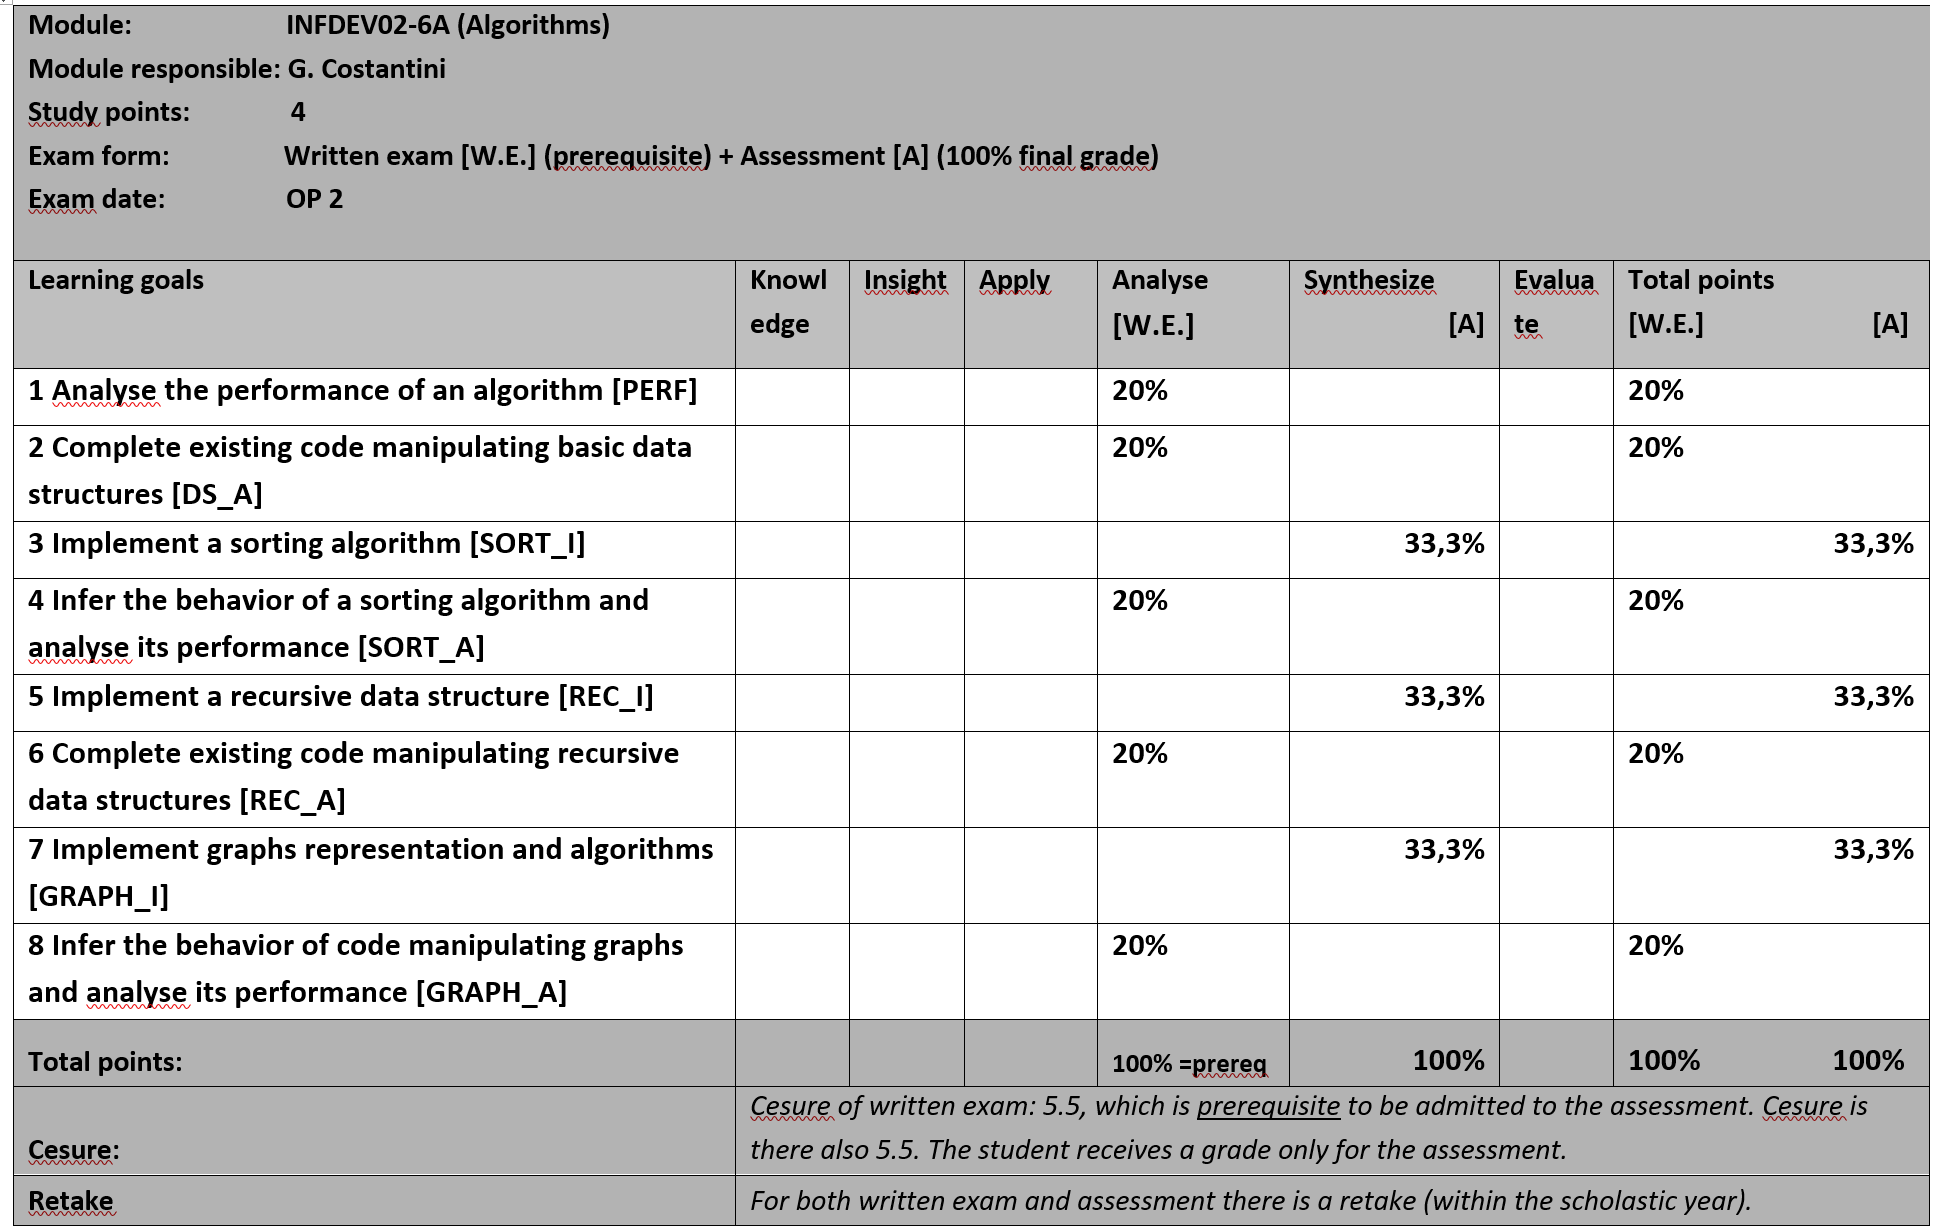
\includegraphics[scale=0.6]{img/toetsmatrijs}
	\caption{Examination matrix of the course}
	\label{img:Ex1}
\end{figure}
\end{comment}

\begin{comment}
\section*{Bijlage 3: Studielast normering in ects}

		Dit hoofdstuk bevat de beschrijving van de procedures om voor beoordeling in aanmerking te komen.\\
		Bijvoorbeeld voldoende aanwezigheid, 80\% van de opdrachten hebben ingeleverd, presentaties hebben verricht etc.\\

		Verder wordt zo gedetailleerd mogelijk beschreven hoe er tot een cijfer wordt gekomen en welke rollen er door docenten en ander betrokkenen hierbij vervuld worden. \\

		Geef een verantwoording van de toets; wat wordt getoetst, waarom is voor deze vorm gekozen.\\

		Vul een toetsmatrijs in voor de toets (zie bijlage).\\

		Beschrijf ook duidelijk de \textbf{herkansingsmogelijkheden}. \\

		Neem in geval van een schriftelijk tentamen een voorbeeldtoets op als bijlage.\\
		Geef daarbij per deelvraag het aantal te verdienen punten aan. \\

		Bij een schriftelijk rapport. Geef de beoordelingscriteria aan met daarbij de mogelijke score en de onderlinge weging. \\

		Toetsduur: \\

		Hoe en wanneer krijgt de student feedback?\\
\end{comment}